% SC4064 --- Chapter 4: Optimization: Occupancy, Latency Hiding and CUDA Streams (0->100)
\chapter{Optimization: Occupancy, Latency Hiding and CUDA Streams}
\label{ch:optimization}
\sloppy

\begin{quote}
\emph{``You cannot make memory faster, but you can make sure the GPU always has something else to do while waiting.''} Occupancy tells you how many warps are available to do that something; streams let you keep the whole system---copy engines, compute, and CPU---busy at once.
\end{quote}

\noindent\fbox{\parbox{\dimexpr\linewidth-2\fboxsep-2\fboxrule}{%
\textbf{From zero: assumes Ch.~1--3.} We know warps, blocks and memory. This chapter asks: how many warps can an SM hold? How does that hide latency? And how do we overlap work that would otherwise serialize? No queuing theory assumed; we derive everything from Little's Law and a picture.}}
\vspace{0.4em}

\section*{Learning Outcomes}
After this chapter you will be able to:
\begin{enumerate}[label=(L\arabic*)]
    \item define occupancy and compute it from registers, shared memory and thread limits;
    \item explain latency hiding via ready warps and why higher occupancy is not always faster;
    \item use Nsight Compute / Occupancy Calculator to spot the limiting resource;
    \item create CUDA streams and overlap host-to-device copy, kernel, and device-to-host copy;
    \item choose block size and launch configuration with a quantitative justification.
\end{enumerate}

% ============================================================
\section{Occupancy: How Many Warps Fit?}
\label{sec:occupancy}
\paragraph{Intuition.} An SM is a hotel: rooms are warps, guests are threads, and amenities are registers and shared memory. Occupancy is the fraction of rooms occupied. A full hotel can always send another guest to the restaurant while one waits for laundry; an empty hotel cannot---the single guest stalls everything.

Formally, for one SM:
\begin{equation}
\text{occupancy} = \frac{\text{active warps}}{\text{max warps per SM}}.
\end{equation}
Max warps is hardware (e.g., 64 on Ampere, i.e., 2048 threads). Active warps is the minimum of four caps: (1) thread cap: $\lfloor2048/B\rfloor\times(B/32)$ warps from $B$ threads/block; (2) block cap: max 32 blocks/SM; (3) register cap: $\lfloor\text{regs per SM}/\text{regs per warp}\rfloor$; (4) shared-memory cap: $\lfloor\text{shared per SM}/\text{shared per block}\rfloor\times(B/32)$. The smallest wins. Increasing $B$ or reducing per-thread registers/shared often raises occupancy---until another cap binds.

\begin{figure}[h]\centering
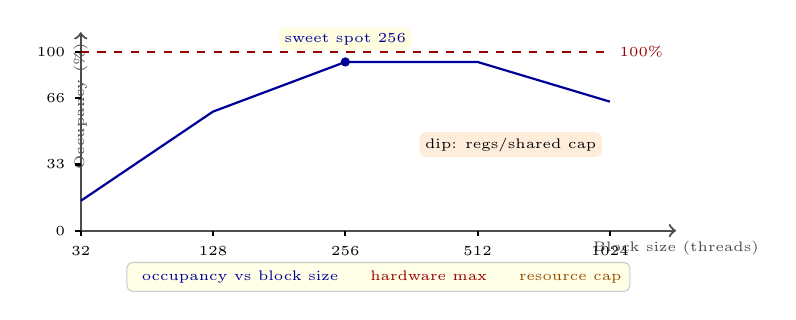
\begin{tikzpicture}[scale=0.84, every node/.style={font=\scriptsize}]
\draw[->, thick, gray!60!black] (0,0) -- (9.0,0) node[below, font=\tiny] {Block size (threads)};
\draw[->, thick, gray!60!black] (0,0) -- (0,3.0) node[left, rotate=90, font=\tiny] {Occupancy (\%)};
% axes ticks
\foreach \x/\lbl in {0/32, 2/128, 4/256, 6/512, 8/1024} {
  \draw[thick] (\x,0) -- (\x,-0.08) node[below, font=\tiny] {\lbl};
}
\foreach \y/\lbl in {0/0, 1/33, 2/66, 2.7/100} {
  \draw[thick] (0,\y) -- (-0.08,\y) node[left, font=\tiny] {\lbl};
}
% occupancy curve: rises then flat then dip due to regs/shared example
\draw[thick, blue!60!black] (0,0.45) -- (2,1.8) -- (4,2.55) -- (6,2.55) -- (8,1.95);
\fill[blue!60!black] (4,2.55) circle (2pt) node[above=4pt, font=\tiny, fill=yellow!12, rounded corners=2pt, inner sep=2pt] {sweet spot 256};
\draw[dashed, red!60!black] (0,2.7) -- (8,2.7) node[right, font=\tiny, text=red!60!black] {100\%};
\node[font=\tiny, fill=orange!14, rounded corners=2pt, inner sep=2pt] at (6.5,1.3) {dip: regs/shared cap};
\node[font=\tiny, align=left, fill=yellow!10, draw=gray!40, rounded corners=2pt, inner sep=3pt] at (4.5,-0.70) {\textcolor{blue!60!black}{$\blacksquare$ occupancy vs block size} \quad \textcolor{red!60!black}{$\blacksquare$ hardware max} \quad \textcolor{orange!60!black}{$\blacksquare$ resource cap}};
\end{tikzpicture}
\caption{Occupancy versus block size for a typical kernel: rises as more warps fill the SM, plateaus at the hardware max, then dips when registers or shared memory per block limit resident blocks.}
\label{fig:occupancy-curve}
\end{figure}

\begin{definition}[Occupancy limiters]
\emph{Register pressure} is registers per thread $\times$ threads per block exceeding the SM file. \emph{Shared-memory pressure} is shared bytes per block $\times$ blocks per SM exceeding the SM budget. Either forces fewer resident blocks and lower occupancy even if threads alone would allow more.
\end{definition}

\begin{example}[Occupancy calculation]
SM: 2048 threads, 64K registers, 100\,KiB shared. Kernel: $B=256$ threads (8 warps), 32 regs/thread, 4\,KiB shared/block. Thread cap: $2048/256=8$ blocks $\to$ 64 warps. Reg cap: $65536/(32\times256)=8$ blocks $\to$ 64 warps. Shared cap: $100/4=25$ blocks but thread cap already 8, so 8 blocks $\to$ 64 warps $\to$ 100\%. If regs rise to 64/thread, reg cap drops to 4 blocks $\to$ 32 warps $\to$ 50\% occupancy.
\end{example}

% ============================================================
\section{Latency Hiding: Why Occupancy Matters (and When It Does Not)}
\label{sec:latency-hiding}
Memory latency $L$ is 300--500 cycles; a warp that issues a global load is not ready for $L$ cycles. If the SM has $W$ warps and each does $C$ cycles of math per load, Little's Law says the SM stays busy when $W\ge L/C + 1$. Doubling $W$ (higher occupancy) doubles the chance a ready warp exists when one stalls.

But occupancy is not performance. A kernel with high instruction-level parallelism (ILP) or many independent instructions per thread can hide latency with few warps. Conversely, pushing occupancy by spilling registers to ``local'' memory (which is DRAM) hurts more than the extra warps help. The correct metric is wall time, not occupancy; use occupancy as a diagnostic, not a goal. Nsight Compute reports ``SM Throughput'' and ``Memory Throughput'' alongside theoretical and achieved occupancy---trust those.

\begin{figure}[h]\centering
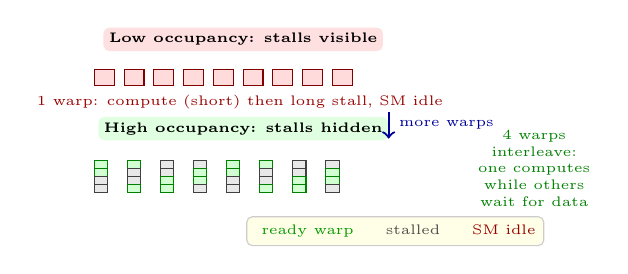
\begin{tikzpicture}[scale=0.84, every node/.style={font=\scriptsize}]
% Timeline: low occupancy vs high occupancy
\node[font=\tiny\bfseries, fill=red!12, rounded corners=2pt, inner sep=2pt] at (2.4,2.6) {Low occupancy: stalls visible};
\foreach \t in {0,0.45,...,3.6} {
  \draw[fill=red!14, draw=red!50!black] (0.15+\t,1.90) rectangle (0.45+\t,2.15);
}
\node[font=\tiny, text=red!60!black] at (2.35,1.65) {1 warp: compute (short) then long stall, SM idle};

\node[font=\tiny\bfseries, fill=green!12, rounded corners=2pt, inner sep=2pt] at (2.4,1.25) {High occupancy: stalls hidden};
\foreach \w in {0,1,2,3} {
  \foreach \t in {0,0.50,...,3.5} {
    \pgfmathparse{mod(\t*2+\w,4) < 2 ? 1 : 0}
    \ifnum\pgfmathresult=1
      \draw[fill=green!18, draw=green!50!black] (0.15+\t,0.65-\w*0.12) rectangle (0.35+\t,0.77-\w*0.12);
    \else
      \draw[fill=gray!18, draw=gray!50!black] (0.15+\t,0.65-\w*0.12) rectangle (0.35+\t,0.77-\w*0.12);
    \fi
  }
}
\node[font=\tiny, text=green!50!black, align=center] at (6.8,0.65) {4 warps\\interleave:\\one computes\\while others\\wait for data};
\draw[->, thick, blue!60!black] (4.6,1.50) -- (4.6,1.10) node[midway, right, font=\tiny] {more warps};
\node[font=\tiny, align=left, fill=yellow!10, draw=gray!40, rounded corners=2pt, inner sep=3pt] at (4.7,-0.30) {\textcolor{green!60!black}{$\blacksquare$ ready warp} \quad \textcolor{gray!60!black}{$\blacksquare$ stalled} \quad \textcolor{red!60!black}{$\blacksquare$ SM idle}};
\end{tikzpicture}
\caption{Latency hiding: with one warp the SM idles during loads; with four warps another ready warp fills each gap. More ready warps $\Rightarrow$ higher utilisation, until math or bandwidth saturates.}
\label{fig:latency-hiding}
\end{figure}

\paragraph{Practical tuning.} Start with $B=128$ or $256$ (multiple of 32, enough warps, not too much shared). Check \texttt{nvcc -Xptxas -v} for regs/thread and shared bytes. Plug into the occupancy calculator (spreadsheet or \texttt{https://xmartlabs.github.io/cuda-occupancy-calculator}) to see the limiter. If shared or regs cap, try \texttt{\_\_launch\_bounds\_\_} or split the kernel. Measure before and after---$10\%$ higher occupancy that costs a spill is a loss.

% ============================================================
\section{CUDA Streams: Overlapping Copy and Compute}
\label{sec:streams}
So far kernels and copies were serial: host-to-device (H2D) $\to$ kernel $\to$ device-to-host (D2H), with the copy engine and compute engine idle in turn. \emph{Streams} are ordered queues; operations in one stream are sequential, but streams run concurrently when hardware allows. With two copy engines (H2D and D2H) plus compute, a three-stage pipeline can overlap.

\begin{figure}[h]\centering
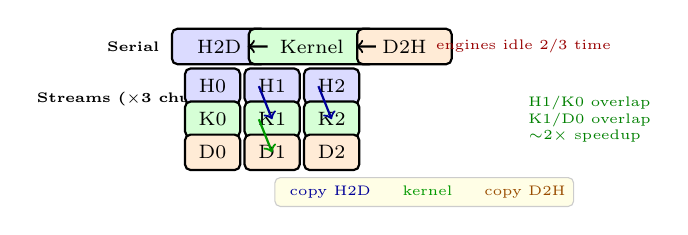
\begin{tikzpicture}[scale=0.84, every node/.style={font=\scriptsize},
  seg/.style={draw, thick, rounded corners=2pt, minimum height=0.45cm, align=center}]
% Serial
\node[font=\tiny\bfseries] at (0.3,2.35) {Serial};
\node[seg, fill=blue!14, minimum width=1.2cm] (s1) at (1.6,2.35) {H2D};
\node[seg, fill=green!16, minimum width=1.6cm] (s2) at (3.0,2.35) {Kernel};
\node[seg, fill=orange!16, minimum width=1.2cm] (s3) at (4.4,2.35) {D2H};
\draw[->, thick] (s1) -- (s2); \draw[->, thick] (s2) -- (s3);
\node[font=\tiny, text=red!60!black] at (6.2,2.35) {engines idle 2/3 time};
% Streamed
\node[font=\tiny\bfseries] at (0.3,1.55) {Streams ($\times$3 chunks)};
\foreach \i in {0,1,2} {
  \node[seg, fill=blue!14, minimum width=0.70cm] at (1.5+\i*0.90,1.75) {H\i};
  \node[seg, fill=green!16, minimum width=0.70cm] at (1.5+\i*0.90,1.25) {K\i};
  \node[seg, fill=orange!16, minimum width=0.70cm] at (1.5+\i*0.90,0.75) {D\i};
}
% overlap arrows
\draw[->, thick, blue!60!black] (2.20,1.75) -- (2.40,1.25);
\draw[->, thick, green!60!black] (2.20,1.25) -- (2.40,0.75);
\draw[->, thick, blue!60!black] (3.10,1.75) -- (3.30,1.25);
\node[font=\tiny, text=green!50!black, align=left] at (7.2,1.25) {H1/K0 overlap\\K1/D0 overlap\\$\sim$2$\times$ speedup};
\node[font=\tiny, align=left, fill=yellow!10, draw=gray!40, rounded corners=2pt, inner sep=3pt] at (4.7,0.15) {\textcolor{blue!60!black}{$\blacksquare$ copy H2D} \quad \textcolor{green!60!black}{$\blacksquare$ kernel} \quad \textcolor{orange!60!black}{$\blacksquare$ copy D2H}};
\end{tikzpicture}
\caption{Streams overlap: serial execution leaves engines idle; chunking data into $N$ pieces and pipelining H2D/Kernel/D2H across streams keeps copy and compute busy together.}
\label{fig:streams-overlap}
\end{figure}

Requirements for overlap: pinned (page-locked) host memory (\texttt{cudaMallocHost} or \texttt{cudaHostAlloc}) for async copies, and async APIs (\texttt{cudaMemcpyAsync}, kernel launch). Default stream (0) synchronises with others unless created with \texttt{cudaStreamNonBlocking}. Events (\texttt{cudaEventRecord} / \texttt{cudaStreamWaitEvent}) express dependencies without host sync.

\begin{lstlisting}[language=C++, caption={Occupancy-aware launch helper and register report.}, label={lst:occupancy}]
#include <cuda_runtime.h>
// Ask compiler to limit registers to raise occupancy (may spill if too low)
__global__ void __launch_bounds__(256, 4) myKernel(float *a, int n){
    int tid = blockIdx.x*blockDim.x + threadIdx.x;
    if(tid<n) a[tid] = a[tid]*2.0f + 1.0f;
}
int main(){
    int B=256; int n=1<<20;
    // compile with: nvcc -Xptxas -v -> reports regs/thread, shared, occupancy
    int minGrid, blockSize;
    cudaOccupancyMaxPotentialBlockSize(&minGrid, &blockSize, myKernel, 0, 0);
    // blockSize is heuristic optimum; measure around it (128,256,512)
    return 0;
}
\end{lstlisting}

\begin{lstlisting}[language=C++, caption={Overlapping copy and compute with two streams and pinned memory.}, label={lst:streams}]
int N=1<<24; size_t bytes=N*sizeof(float);
float *h_a, *d_a;
cudaMallocHost(&h_a, bytes);      // pinned: async copies can overlap
cudaMalloc(&d_a, bytes);
cudaStream_t s0,s1;
cudaStreamCreate(&s0); cudaStreamCreate(&s1);
int chunk = N/2;
for(int i=0;i<2;i++){
    float *h_chunk = h_a + i*chunk;
    float *d_chunk = d_a + i*chunk;
    cudaMemcpyAsync(d_chunk, h_chunk, chunk*sizeof(float),
                    cudaMemcpyHostToDevice, i==0?s0:s1);
    myKernel<<< (chunk+255)/256, 256, 0, i==0?s0:s1 >>>(d_chunk, chunk);
    // D2H similarly; use cudaEventRecord / cudaStreamWaitEvent for deps
}
cudaDeviceSynchronize(); // wait for both streams
cudaFreeHost(h_a); cudaFree(d_a);
\end{lstlisting}

\paragraph{When streams help.} Overlap hides H2D/D2H time only if kernel time $\approx$ copy time; if the kernel dominates, overlap is minor. Chunking also improves load balance across SMs. For multi-GPU, streams plus \texttt{cudaMemcpyPeerAsync} overlap inter-GPU transfers similarly (preview of Ch.~7).

% ============================================================
\section{Exercises}
\label{sec:ch04-exercises}
\begin{enumerate}[label=E4.\arabic*, leftmargin=*, itemsep=0.6em]
    \item \textbf{Occupancy math.} SM: 2048 threads, 64K regs, 96\,KiB shared, max 32 blocks. Kernel A: $B=128$, 32 regs/thread, 2\,KiB shared/block. Kernel B: $B=256$, 48 regs/thread, 8\,KiB shared/block. Compute occupancy for each and name the limiter. Which would you tune first?
    \item \textbf{Latency hiding estimate.} Global latency $L=400$ cycles, each thread does $C=8$ math cycles per load, 4 warps resident. Is the SM fully utilised? How many warps needed for 100\%? If you double $C$ via ILP (unrolling), how does the requirement change?
    \item \textbf{Block-size sweep.} You measure kernel time for $B=32,64,128,256,512,1024$ and get 12, 8, 6, 5.5, 6.2, 7.1\,ms. Explain the U-shape: why does tiny $B$ hurt, why does huge $B$ hurt despite higher occupancy? What would you pick and why?
    \item \textbf{Streams correctness.} Two streams copy chunks 0 and 1 and launch kernels K0, K1 that read their chunk. Without events, can K1 start before H2D of chunk 1 finishes? Can K0 read chunk 1? Draw the dependency graph and add one event to enforce ``H1 before K1'' without serialising streams.
    \item \textbf{Pinned memory.} Why does \texttt{cudaMemcpyAsync} require pinned host memory to overlap? What happens if you use pageable memory or forget \texttt{cudaStreamNonBlocking}? Quantify: pageable copy pins on the fly at $\sim$6\,GB/s vs.\ pinned at $\sim$25\,GB/s PCIe4---how does this affect overlap benefit?
\end{enumerate}

\paragraph{Putting it together.} A good optimisation workflow is: (1) profile baseline with Nsight Systems (see batch vs.\ stream timeline, copy/compute overlap). (2) Check Nsight Compute occupancy and limiter. (3) Fix the limiter (adjust $B$, reduce regs/shared, or accept lower occupancy if ILP is high). (4) Chunk work and add streams where copy time matters. (5) Re-measure; if occupancy rose but time did not, you chased the wrong metric---go back to the Roofline.

\begin{remark}[Rules of thumb that survive]
Small blocks (64--128) rarely saturate; huge blocks (1024) often exhaust regs/shared and hurt flexibility. $256$ is a reliable default---measure one step either side. Pinned memory + two streams + double-buffering is the simplest overlap that wins on most PCIe-bound workloads. For compute-bound kernels, overlap barely helps; spend time on coalescing and bank conflicts (Ch.~3) instead.
\end{remark}

\smallskip

% optimisation checkpoint: occupancy + streams mastered

% ============================================================
\section*{Chapter Notes}
Occupancy, \texttt{\_\_launch\_bounds\_\_} and the calculator are documented in CUDA C++ Programming Guide \S7 and CUDA Toolkit ``Occupancy Calculator'' (spreadsheet and runtime API \texttt{cudaOccupancy*}). Little's Law treatment follows Volkov, \emph{Better performance at lower occupancy} (GTC 2010) and the ``Latency hiding'' note in Guide \S7. Streams, events and async copies: Guide \S3.2.5--3.2.6 and Wilt, \emph{The CUDA Handbook} (2nd ed., 2013, Ch.~7). Profiling: Nsight Compute (``Occupancy'', ``SM Throughput'') and Nsight Systems (stream timeline). For deeper overlap see Ch.~7 on multi-GPU and cooperative groups.
% End of Chapter 4
